\lecture{25}{2025-05-19}{Intégrales sur intégrales}{}


\begin{parag}{Exemple}
	$D = \left\{(x, y) \in \mathbb{R}^{2}: 1 < x < 2, \frac{1}{x} < y  < x \right\}$ avec la fonction $f\left(x, y\right) = x + \frac{1}{y}$ Nous cherchons donc:
	\begin{align*} \int\int_D f(x, y)dxdy = ? \end{align*}
	Comme on peut le voire, notre ensemble est dejà une intégrale de type 1. On obtient:
	\begin{align*} \int_1^2 \left( \int_{\frac{1}{x}}^x x + \frac{1}{y}dy \right) dx &= \int_1^2dx \int_{\frac{1}{x}}^x x + \frac{1}{y}dy\\
	&= \int_1^2dx (xy + \ln y)\mid_{\frac{1}{x}}^x\\
	&= \int_1^2 x^2 + \ln x - 1 - \ln \frac{1}{x} dx\\
	&= \int_1^2 x^2 + 2\ln x - 1 dx =  \frac{1}{3}x^3 - x \mid_1^2 + 2 \int_1^2 \ln x dx \\
	&= \frac{8}{3} -2 - \frac{1}{3} + 1 + 2x\ln x \mid_1^2 - 2\int 1dx\\
	&= \frac{7}{3} - 1 + 4\ln 2 - 2x\mid_1^2 = \frac{7}{3} - 1 + 4\ln 2 - 4 + 2 = -\frac{2}{3} + 4 \ln 2 > 0
	\end{align*}
\end{parag}

\begin{parag}{Changement d'ordre par intégration}
    Donc si maintenant on veut le faire dans l'autre sens, on veut écrire $x$ dans les bornes de $y$.\\
    On cherche en premier lieu l'intersection les deux intersections de $D: y = x$ et $y =  \frac{1}{x}$:
    \begin{align*} 
	    \frac{1}{x} =  x \implies x^2 = 1, x > 0 \implies x =  1, y = 1
    \end{align*}
    On a donc le max qui est $x =  2= y$ ce qui nous donne:
    \begin{align*} D_1 = \{1 < y < 2, \mathspace y < x < 2\}\\
	    D_2 =  \{\frac{1}{x} < y < 1, \frac{1}{y} < x < 2\}
    \end{align*}
    Qui sont donc les deux de types $2$. Si on écrit donc l'intégrae:
    \begin{align*} 
	    \int_{\frac{1}{2}}^1 \left(\int_{\frac{1}{y}}^2 x + \frac{1}{y}dx\right) dy + \int_1^2 \left(\int_y^2 x + \frac{1}{y}dx\right) dy
    \end{align*}
\end{parag}




\begin{parag}{Exemple 2}
	Soit $D = \{ \left(x, y\right) \in \mathbb{R}^{2}: 0 < y < 1, 0 < x < \arccos y\}$.\\
	Calculer $\int\int_D xdxdy \implies D = \{\left(x, y\right) \in\mathbb{R}^{2}:0 < x < \frac{\pi}{2}, 0 < y < \cos x\}$ Ce que l'on peut aisément intégrer:
	\begin{align*} 
		\int_0^{\frac{\pi}{2}}dx \int_0^{\cos x}xdy &= \int_0^{\frac{\pi}{2}}dx (xy\mid_0^{\cos x})\\
							    &= \int_0^{\frac{\pi}{2}}x \cos x dx = \int_0^{\frac{\pi}{2}} \underbrace{x}_{f}d \underbrace{\sin x}_{g}\\
							    &= x\sin x \mid_0^{\frac{\pi}{2}} - \int_0^{\frac{\pi}{2}}\sin x dx\\
							    &= \frac{\pi}{2} - 1
	\end{align*}
	Maintenant on peut le faire dans l'autre sens:
	\begin{align*} 
		\int\int_D x dxdy &= \int_0^1 dy \int_0^{\arccos y}xdx\\
				  &= \int_0^1 dx (\frac{1}{2}x^2 \mid_0^{\arccos y})\\
				  &= \frac{1}{2} \int_0^1 (\arccos y)^2 dy\\
				  &= \frac{1}{2}\int_{\frac{\pi}{2}}^0 u^2 d \cos u\\
				  &= \frac{1}{2} u^2 \cos u \mid_{\frac{\pi}{2}}^0 - \frac{1}{2}\int_{\frac{\pi}{2}}^0 2u \cos u du \\
				  &= 0 - \int_{\frac{\pi}{2}}^0 u d \sin u = -u \sin u\mid_{\frac{\pi}{2}}^0 - \int_{\frac{\pi}{2}}^0\sin u du = \frac{\pi}{2} - 1
	\end{align*}
	Comme on le voit ici, ça vaut la peine de refléchir quel type utiliser avant de commencer à calculer.
\end{parag}


\subsection{Théorème de Fubini pour les intégrales triples}
\begin{parag}{Théorème}
   \begin{theoreme}
	   Soit $\left[a, b\right]$ intervalle, $a < b$; $\phi_1, \phi_2: \left[a, b\right] \to \mathbb{R}$ continues $\phi_1\left(x\right) < \phi_2 \left(x\right) \forall x \in ] a, b [$.
	   \begin{align*} D = \left{(x, y) \in \mathbb{R}^{2}: a < x < b, \mathspace \phi_1(x) < y < \phi_2(x)\right} \end{align*}
	   Soient $G_1, H : \overline{D} \to \mathbb{R}$ continues, tel que $G\left(x, y\right) < H\left(x, y\right) \mathspace \forall \left(x, y\right) \in D$.\\
	   \begin{align*} E =  \{(x, y, z) \in \mathbb{R}^{3}: (x, y) \in D; \mathspace G(x, y) < z < H(x, y)\} \end{align*}
	   Soit $f : \overline{E} \to \mathbb{R}$ continue,\\
	   Alors $f$ est intégrable sur $E$ et on a:
	   \begin{align*} 
		   \int\int\int_E f(x, y, z) dxdydz =  \int_a^b \left(\int_{\phi_1(x)}^{\phi_2(x)}\left(\int_{G(x, y)}^{H(x, y)}f(x, y, z)dz\right)dy\right)dx
	   \end{align*}
   \end{theoreme} 
\end{parag}

\begin{parag}{Exemple}
	Soit $E = \{\left(x, y, z\right) \in \mathbb{R}^{3}: 0 < z < y < x < 1\} \implies \int\int\int_E f\left(x, y, z\right)dxdydz =$  Avec la fonction $f\left(x, y, z\right) = e^{x^3}$\\
	On cherche donc à écrire nous ensemble petit à petit. On sait déjà que $0 < x < 1$ et que $0 < y < x$, et que $0 < z < y$ (c'est comme si on séparait notre inégalité).
	Ce qui nous donne comme domaine:
	\begin{align*} E = {(x, y) \in \mathbb{R}^{3}, 0 < x < 1, 0 < y < x, 0 < z < y} \end{align*}
	\begin{center}
	    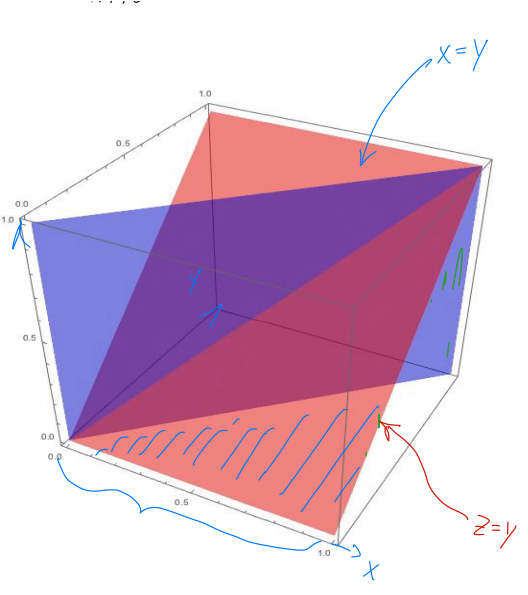
\includegraphics[scale=0.8]{12025-05-19.png}
	\end{center}
	

	On nous donne donc comme intégrale:
	\begin{align*} 
		\int\int\int_E f(x, y, z)dxdydz &= \int_0^1dx \int_0^x dy \int_0^y e^{x^3}dz\\
						&= \int_0^1 dx \int_0^x dy ze^{x^3}\mid_0^y\\
						&= \int_0^1 dx \int_0^x y e^{x^3}dy \\
						&= \int_0^1 dx \int_0^x y e^{x^3}dy = \int_0^1dx \cdot  \frac{1}{2}y^2 e^{x^3}\mid_0^x\\
						&= \frac{1}{2}\int_0^1x^2 e^{x^3}dx = \frac{1}{6}\int_0^1 e^{x^3}d(x^3) = \frac{1}{6}e^{x^3}\mid_0^1 =  \frac{1}{6}(e-1)
	\end{align*}
	Donc maintenant si on veut le faire dans l'autre sens (avec le $z$ en avant dernier) on a:
	\begin{align*} E = {(x, y, z) \in \mathbb{R}^{3}: 0 < x < 1, 0 < z < x, z < y < x} \end{align*}	
	On peut jouer dans l'ordre de nos ensemble, on voit ici qu'il y a $6$ possibilités d'arranger l'ensemble, dont toute donne la même réponse.
	\begin{center}
	    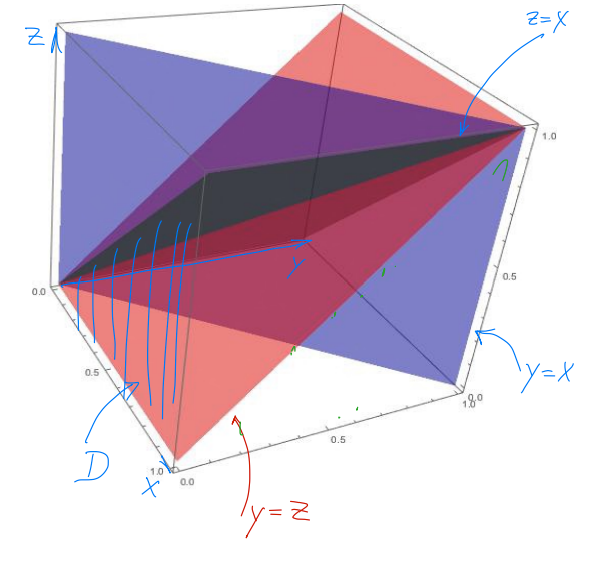
\includegraphics[scale=0.8]{22025-05-19.png}
	\end{center}
\end{parag}
\begin{parag}{Exemple 4}
	Trouver le volume de la région $E \subset \mathbb{R}^{3}$ entre les plans $x =  0,  y = 0, z= 0$ et $2x + 3y - z =  6$.\\
	Donc déjà, on a $4$ plans, ce qui nous donnera dans notre cas un triangle. On cherche donc les arrêtes de se triangle (l'intérsection de deux plans ensemble) on a:
	\begin{align*} z =  0 \implies 2x + 3y = 6 \implies y =  2 -\frac{2}{3}x \end{align*}
	On a donc ensuite l'intersection de tout les plans:
	\begin{align*} x = 0, y = 0, z = 2x + xy - 6 \implies -6 \end{align*}
	On a donc:
	\begin{align*} E = \{0 < x < 3, 0 < y < 2- \frac{2}{3}x, 2x + 3y - 6 < z < 0\} \end{align*}
	Pouruoi dans ce sens? étant donnée que notre plan se trouve en dessous de 0, il est forcémment borné supérieurement par ce dernier.\\
	Si on calcule donc le volume:
	\begin{align*} 
		V &= \int\int\int_E 1 dxdydz = \int_0^3dx \int_0^{2 - \frac{2}{3}x}dy \int_{2x + 3x - 6}^0\\
		  &= \int_0^3dx \int_0^{2 - \frac{2}{3}x}(-2x - 3y + 6)dy\\
		  &= \int_0^3dx \int_0^{2 - \frac{2}{3}x}(-2x - 2y + 6)dy =  \int_0^3dx (-2xy - \frac{3}{2}y^2 + 6y) \mid_0^{2 - \frac{2}{3}x}\\
		  &= \int_0^3 (-2x(2 - \frac{2}{3}x)- \frac{3}{2}(2- \frac{2}{3}x)^2 + 6(2 - \frac{2}{3}x))dx \\
		  &= \int_0^3 -4x + \frac{4}{3}x^2 - 6 + 4x - \frac{2}{3}x^2 + 12 - 4x dx\\
		  &= \int_0^3 - 4x + \frac{2}{3}x^2 + 6 dx = -2x^2 + \frac{2}{9}x^3 + 6x \mid_0^3 =  6
	\end{align*}
\end{parag}



\subsection{Changement de variables dans une intégrale multiple}
\begin{theoreme}

Soit $E \subset \mathbb{R}^{n}$ un sous-ensemble ($\overline{E}$ compact); $\psi: E \to \mathbb{R}^{n}$ telle que $\psi \in C'\left(E\right)$ et $\psi: E \to \psi\left(E\right)$ est bijective ($J_\psi\left(\overline{u}\right)$ est invertible $\forall \overline{u} \in E$).\\
Soit $f: \overline{D} = \overline{\psi\left(E\right)} \to \mathbb{R}$ une fonction continue.\\
Alors:
\begin{align*} \int_D f(\overline{x})d\overline{x} = \int_E f(\psi(\overline{u})) \cdot  \left|\det J_{\psi} (\overline{u})\right|d\overline{u} \end{align*}
\end{theoreme}
\begin{parag}{Example 0}
    On prends $f\left(x,y\right) = 1 =  f\left(u, v\right)$.\\
    Soit donc:
    \begin{align*} \psi (u, v) =  \begin{pmatrix} 3u \\ 2b \end{pmatrix}  = \begin{pmatrix} x \\ y \end{pmatrix} \text{ de classe } C^1 \end{align*}
    \begin{align*} J_\psi (u, v) = \begin{pmatrix} 3 & 0 \\ 0 & 2 \end{pmatrix}  \implies \left|\det J_\psi \left(u, v\right)\right|= 6 \end{align*}
    
\end{parag}
\begin{parag}{Exemple 5}
	Soit $f\left(x,y\right) =  x^2$, $D =  \{\left(x,y\right) \in \mathbb{R}^{2}; 0 < x <1, -x < y < x\} \bigcup \{\left(x, y\right) \in \mathbb{R}^{2}: 1 < x < 2, x - 2 < y < 2 - x\}$.\\
	On calcule l'intégrale:
	\begin{align*} 
		\int \int_D f(x, y) dxdy =  \int_0^1 dx \int_{-x}^x x^2 dy + \int_1^2dx \int_{x-2}^{2-x}x^2dx
	\end{align*}
	Ou alors:
	\begin{align*} 
		\begin{cases}
		    u 2
		\end{cases} \implies
		E =  
		\begin{cases}
			(u, v) :  0 < u < 2\\ 0 < v < 2
		\end{cases} =
	\begin{cases}
	    x = \frac{1}{2}(u + v)\\ y =  \frac{1}{2}(u-v) 
	\end{cases}
	\end{align*}
	On a donc pour la jacobienne:
	\begin{align*} J_{\psi(u, v)} =  \begin{pmatrix} \frac{1}{2} &- \frac{1}{2} \\\frac{1}{2}  & \frac{1}{2} \end{pmatrix}  \implies \det J_{\psi (u, v)} =  \frac{1}{2}\end{align*}
	Ceux qui nous donne lorsqu'on calcule l'intégrale (attention à ne pas oublié le facteur du déterminant):
	\begin{align*} \int\int_D x^2dxdy =  \int\int_E (\frac{1}{2}(u + v))^2 \cdot  \frac{1}{2}dudv\\
		&= \int_0^2 dv \int_0^2 (\frac{1}{8}(u + v)^2)du\\
		\int_0^2 dv (\frac{1}{24}(u + v)^3\mid_0^2)\\
		&= \int_0^2 \frac{1}{24}((v + 2)^3 - v^3) dv\\
		&=  \frac{1}{24}\frac{1}{4} ((v + 2)^4 - v^4)\mid_0^2\\
		&= \frac{7}{3}
	\end{align*}
\end{parag}


